\documentclass[10pt]{article}

\usepackage{lipsum}
\usepackage{url}
\usepackage{float}
\usepackage{amsmath}
\usepackage{enumitem}
\usepackage{graphicx}
\usepackage{caption}
\usepackage{subcaption}
\usepackage{rotating}
\usepackage{geometry}
\usepackage{listings}
\usepackage{hyperref}
\usepackage[T1]{fontenc}
\usepackage[numbered]{matlab-prettifier}

\newcommand{\documentTitle}{Lab 6 - Digital Signal Processing}
\newcommand{\documentAuthor}{Andrew Pham, Aneel Damaraju}
\newcommand{\courseTitle}{ELEC 240}
\newcommand{\testDate}{October 16, 2018}
\newcommand{\reportDate}{October 23, 2018}

\geometry{margin=1in}
\lstset{
    tabsize=4,
    basicstyle={\ttfamily},
    captionpos=b,
    belowskip=1em,
    aboveskip=1em,
    numbers=left,
	escapechar=\@,
}

\title{
    \textbf{\courseTitle} \\
    \textbf{\documentTitle} \\
    \bigskip
    \textbf{\large{Test performed: \testDate}} \\
    \textbf{\large{Report submitted: \reportDate}} \\
    \bigskip
    \bigskip
}
\author{\documentAuthor}
\date{}

\begin{document}

\maketitle

\newpage

\section{Objective}



\medskip

%\textit{Note (To be deleted): Think of this test report as a document with your peers as your readers. This means you can assume a similar knowledge background as you. Your readers should be able to easily understand what is going on, and also be able to repeat your lab results based on your document and all references you cite.}

%\textit{For the Objective section, identify the test you performed and its objectives. The objectives of the test are important to state because they are usually analyzed in the conclusion to determine whether the test succeeded.}

\section{Materials}

Your text here

\medskip

\textit{Note (To be deleted): Provide a bullet point list of components, software tools, and hardware (such as the NI VirtualBench or DMM) used during the lab}

\section{Test Description}

Your text here

\medskip

\textit{Note (To be deleted): This section provides a summary of the test your team performed. Give enough information so readers can understand what you did, but do not go into the details of every step.}

\subsection{Pre-Lab Calculations and Schematics}

Your text here

\medskip

\textit{Note (To be deleted): Include the homework pre-calculations and schematics that serve as the initial setup for the test. Briefly explain the importance of each item you include. You may want to number your equations/figures so you can refer to them in later sections. Including photos of handwritten work is okay.}

\section{Results and Discussion}

In Experiment 6.1, Part A, we explored sampling a signal in the time domain. We began by connecting the function generator to pin 46, which was the input to the LabView software and generated a 5 $V_{pp}$, 300 Hz sine wave. We then sampled the signal at a rate of 10000 samples per second with average set to RMS averaging to achieve the following waveform graph in Fig \ref{fig:firstsample} below. 

\begin{centering}
	\begin{figure} [H]
		\centering
		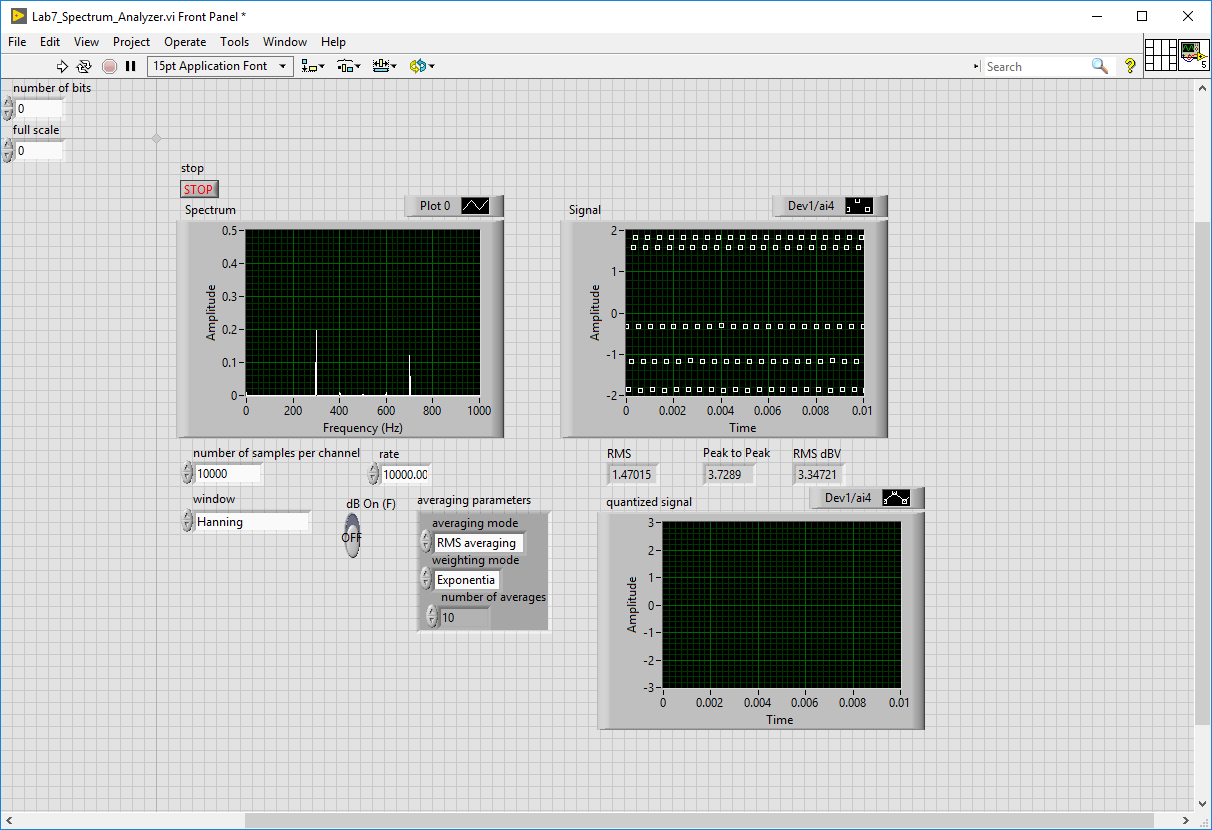
\includegraphics[scale=0.22]{images/61a2khzsample.PNG}
		\caption{Sample of 5 $V_{pp}$, 300 Hz Sine Wave}
		\label{fig:firstsample}
	\end{figure}
\end{centering}

We then began to increase the frequency of the sine wave outputted by the function generator. When the output frequency was half of the sampling frequency, we observed that the samples alternated between positive and negative values. We began to observe aliasing past 5kHz, and the input frequency stopped matching the displayed frequency in Labview. For example, in Fig \ref{fig:11khz} and Fig \ref{fig:13khz} below, we can observe aliasing when the input frequency is 11 kHz and 13 kHz, respectively. 

\begin{centering}
	\begin{figure} [H]
		\centering
		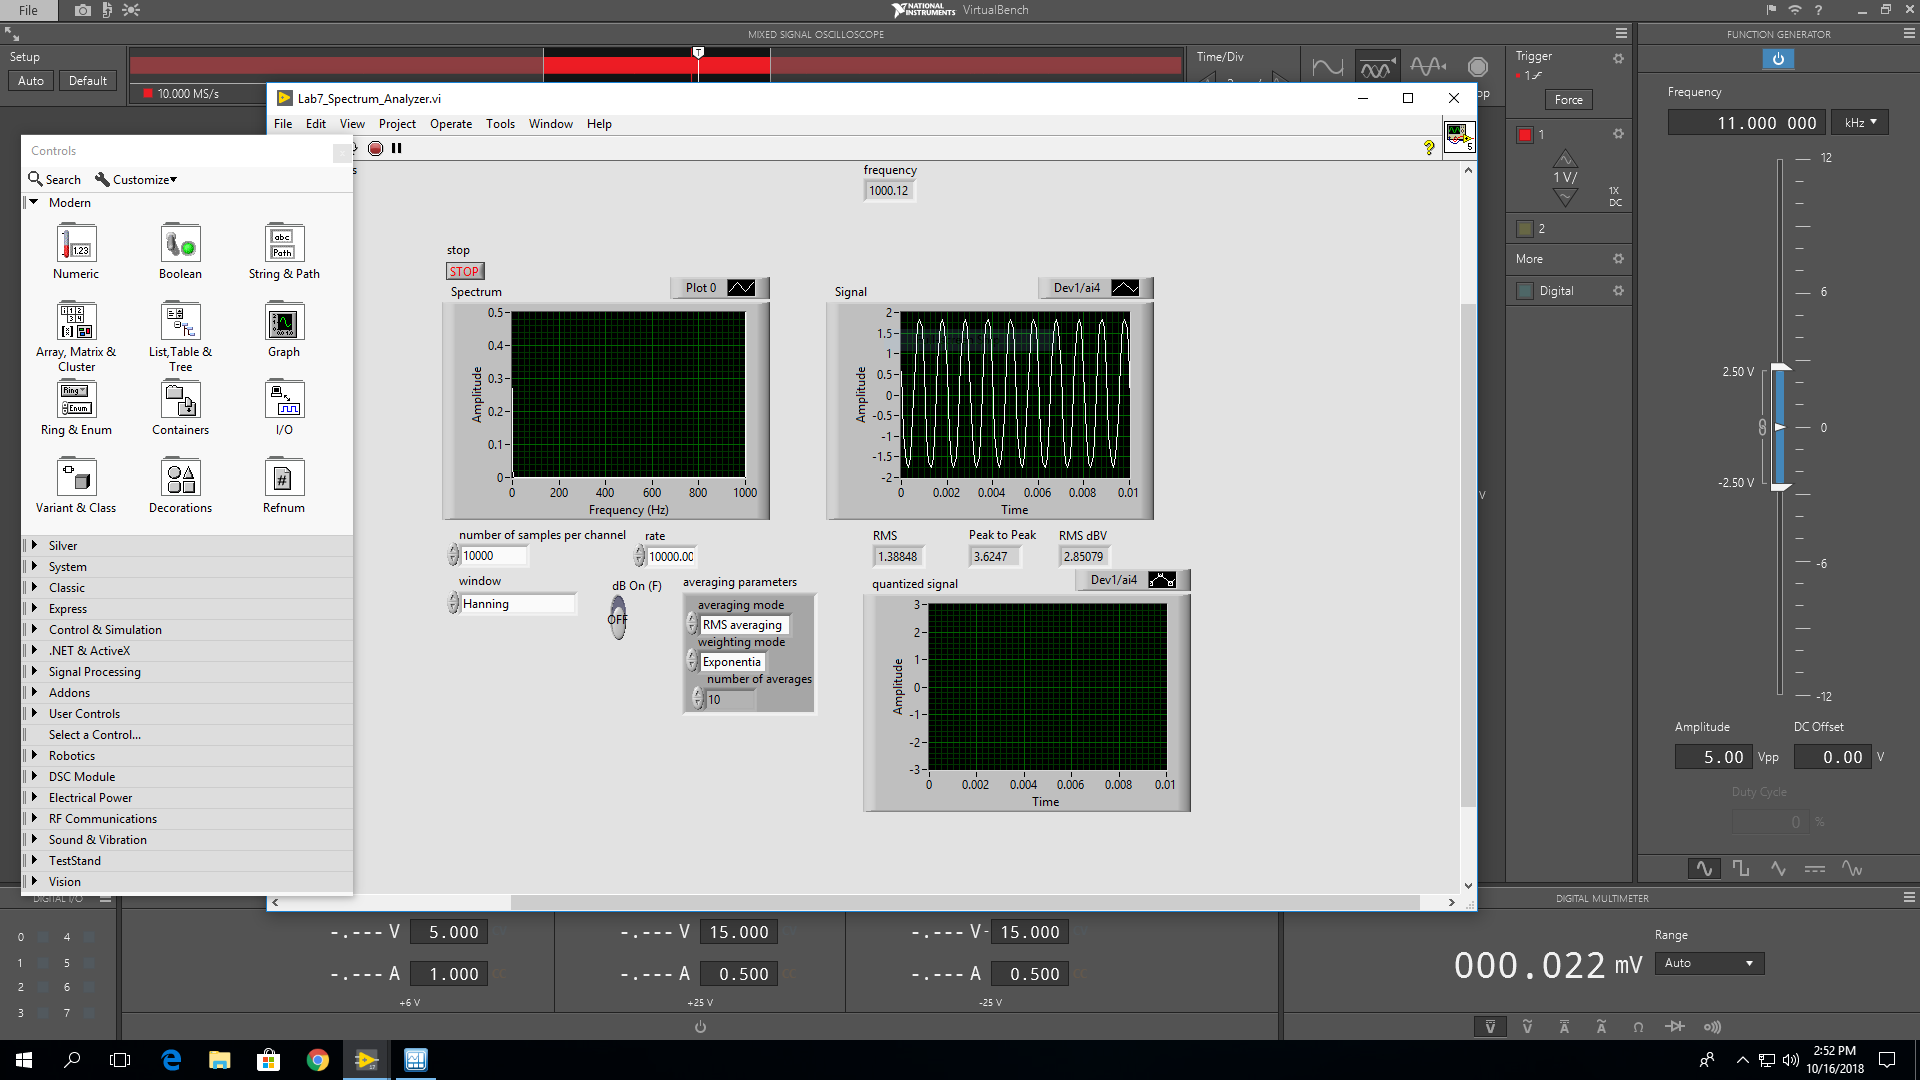
\includegraphics[scale=0.22]{images/51a11000input1000measured.PNG}
		\caption{10 kHz Sample of 11kHz Sine Wave}
		\label{fig:11khz}
	\end{figure}
\end{centering}

\begin{centering}
	\begin{figure} [H]
		\centering
		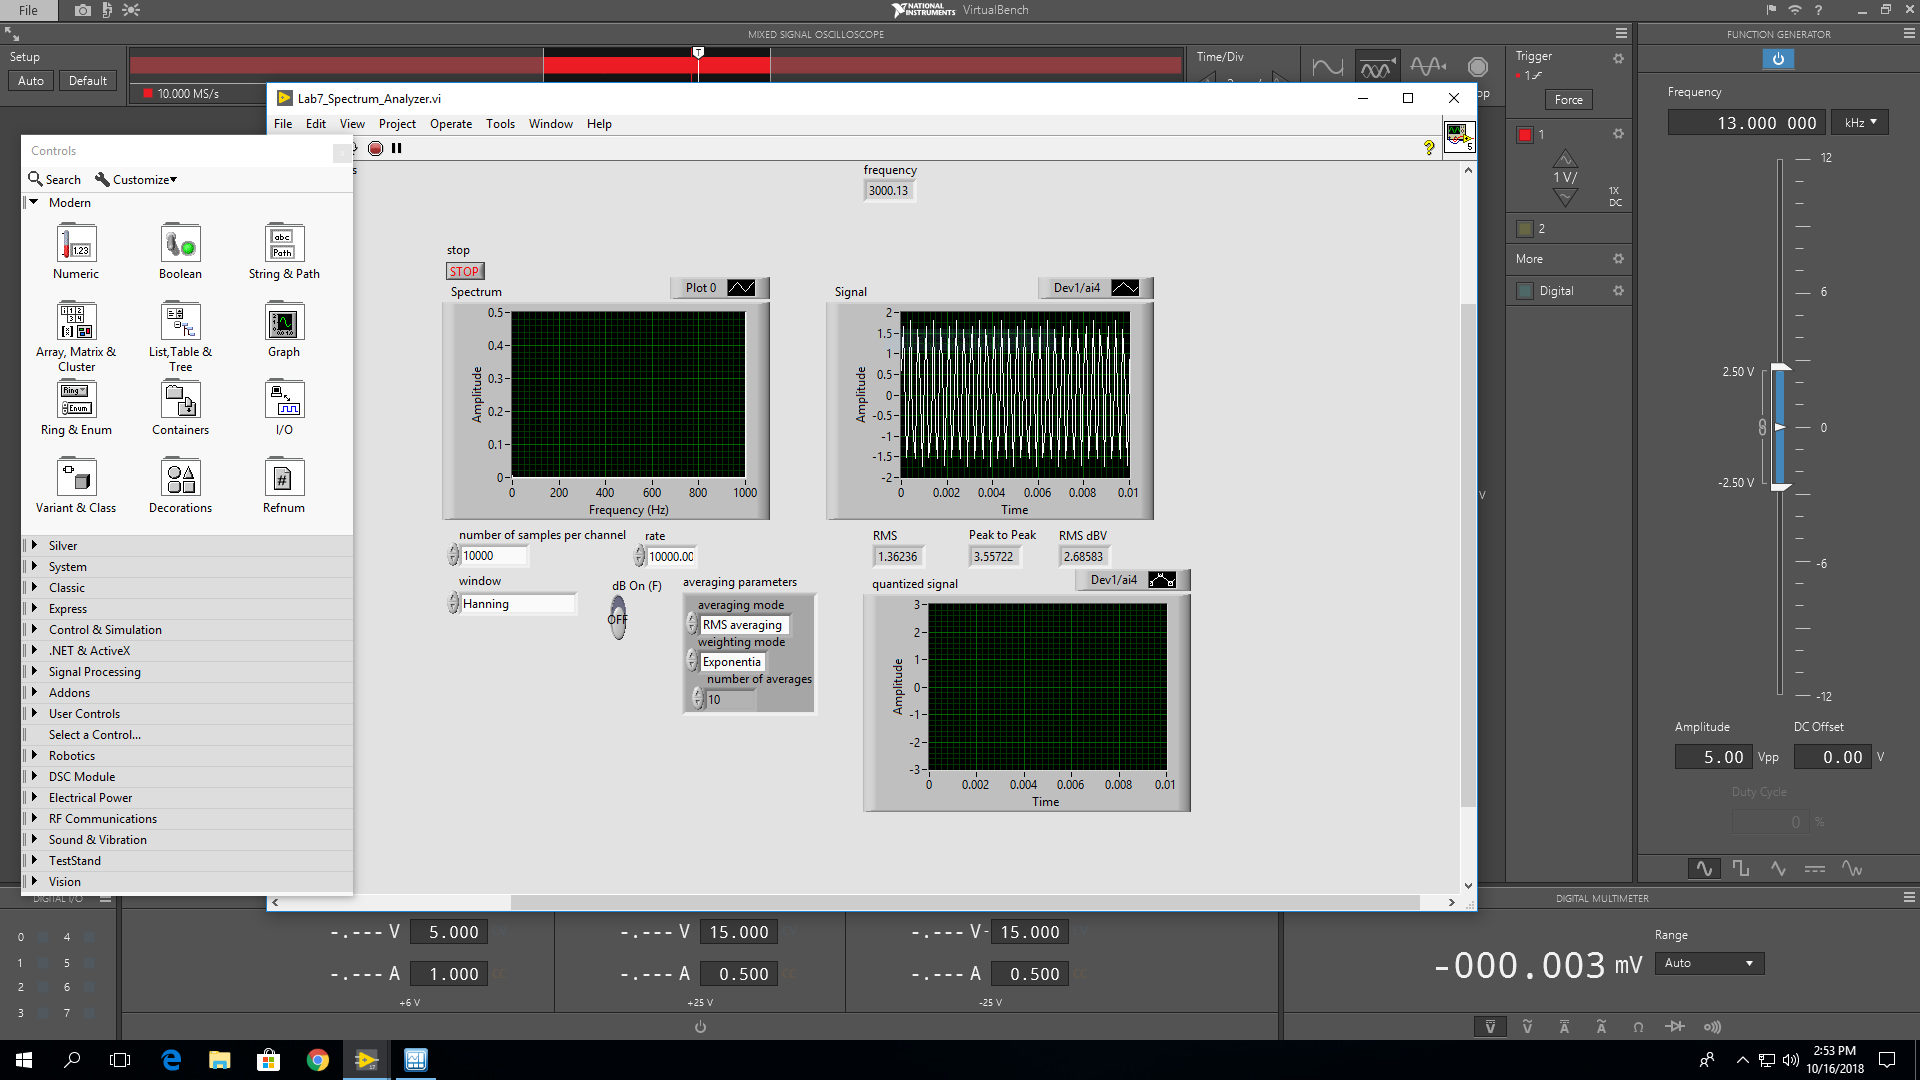
\includegraphics[scale=0.22]{images/51a13000input3000measured.PNG}
		\caption{10 kHz Sample of 11kHz Sine Wave}
		\label{fig:13khz}
	\end{figure}
\end{centering}

In the above figures, the output waveform is the alias of the input frequency, which occurs whenever twice the input frequency exceeds the sampling frequency. This concept is directly related to the Nyquist criterion, which states that no aliasing will occur as long as the sampling frequency is greater than or equal to twice the input frequency. Whenever the input frequency exceeds the Nyquist frequency, the input frequency is "folded over" into a lower. Thus, the 11 kHz signal was folded over the 10 kHz sampling frequency into a 1 kHz wave, and the 13 kHz signal was folded over the 10 kHz sampling frequency into a 3 kHz wave, as seen in the figures above. 

We then switched the function generator to produce a square wave and a sine wave. On frequencies that were integer divisors of the sampling frequency, the wave appeared to be sampled correctly below 5 kHz. However, on other frequencies such as 1.3 kHz, both the triangle and square wave appeared distorted. We attribute this distortion to the fact that neither square waves nor triangle waves are bandlimited, which means that the Nyquist Sampling theorem does not apply to them.


In Part B of Experiment 6.1, we explored amplitude quantization of discretely sampled signals. We began by producing a 1 kHz sine wave and feeding it into the amplitude quantizer that we constructed in Labview. As we increased the number of bits used by the quantizer, we noticed that the sampled sine wave became much more fluid and discerniblee. Likewise, as we decreased the number of bits, the sampled sine waveform became choppier and more step-like. We then switched the power spectrum graph to accept the discretely quantized sine wave as input rather than the original analog sine wave. We noticed that the amplitude of the power spectrum graph increased by 20\%. 

\section{References}

Your text here

\medskip

\textit{Note (To be deleted): List any datasheets, websites, lab procedure, etc. used during the lab.}

\section{Conclusion}

Your text here

\medskip

\textit{Note (To be deleted): While the ``Results and Discussion'' section focused on the test results individually, the ``Conclusion'' discusses the results in the context of the entire experiment. Usually, the objectives given in the ``Introduction'' are reviewed to determine whether the experiment succeeded. If the objectives were not met, you should analyze why the results were not as predicted.}

\section{Errors}

Your text here

\medskip

\textit{Note (To be deleted): Briefly list sources of error and discuss how to eliminate or deal with them}

\end{document}
